\question Draw an environment diagram for the following code:

\begin{lstlisting}
def rec(x, y):
    if y > 0:
        return x * rec(x, y - 1)
    return 1
rec(3, 2)
\end{lstlisting}
Bonus question: what does this function do?

\textit{Note: This problem is meant to help you understand what really goes on when we make the "recursive leap of faith".
However, when approaching or debugging recursive functions, you should avoid visualizing them in this way.}

\begin{center}
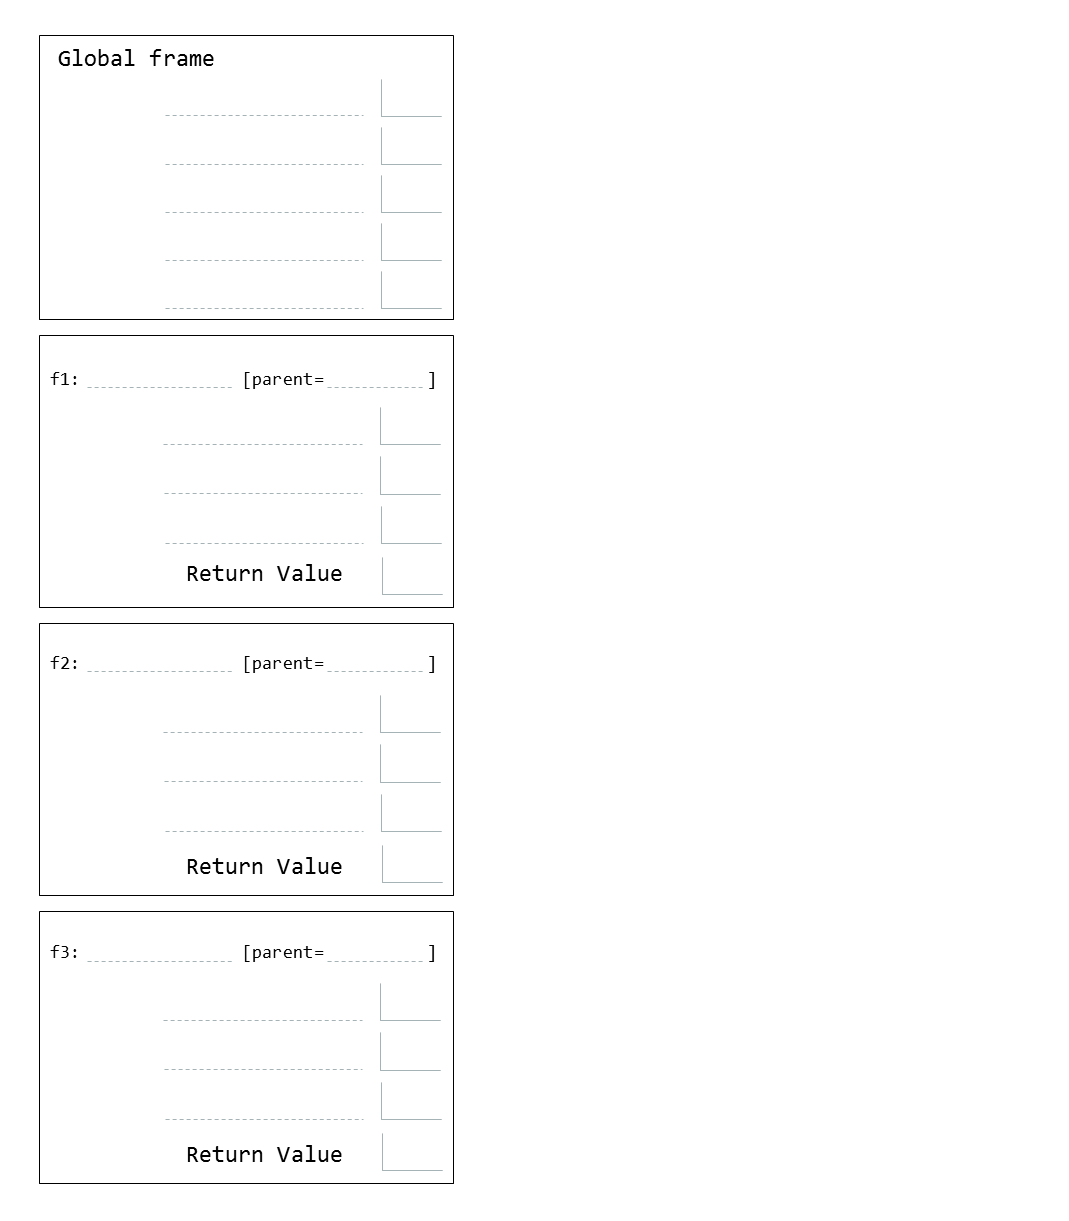
\includegraphics[scale=.5]{env-diagram-template.png}
\end{center}

\begin{blocksection}
\begin{solution}[0in]
\begin{center}
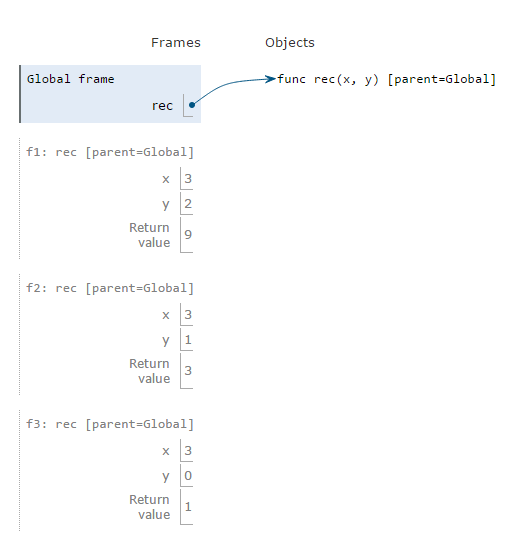
\includegraphics[scale=.8]{env-diagram-solution.png}
\end{center}
This function computes {\tt x ** y}. \\
\href{https://www.youtube.com/watch?v=n2Hq5EWuBGY&t=0s&list=PLx38hZJ5RLZd35oDi3TGz5p9DyyxU3WwA&index=3}{Video Walkthrough}
\end{solution}
\end{blocksection}
